\chapter{Polyhedron's dimension}

    \prob{
        Give an algorithm based in simplex to compute the dimension of a Polyhedron.
    }
    
    \begin{proof}
        First of all, we are going to try to get rid of degenerated vertices. And we always can do this
        by cutting off the corners.\pn

        A degenerated vertex is when it satisfies too much thight restrictions, that is, in other words,
        that we have uneccesary restrictions, or in mathematical speach, that these restrictions are
        linearly dependent.\pn

        As an example of degenerated vertex, you can take a look at the next figure.\pn

        \begin{center}
            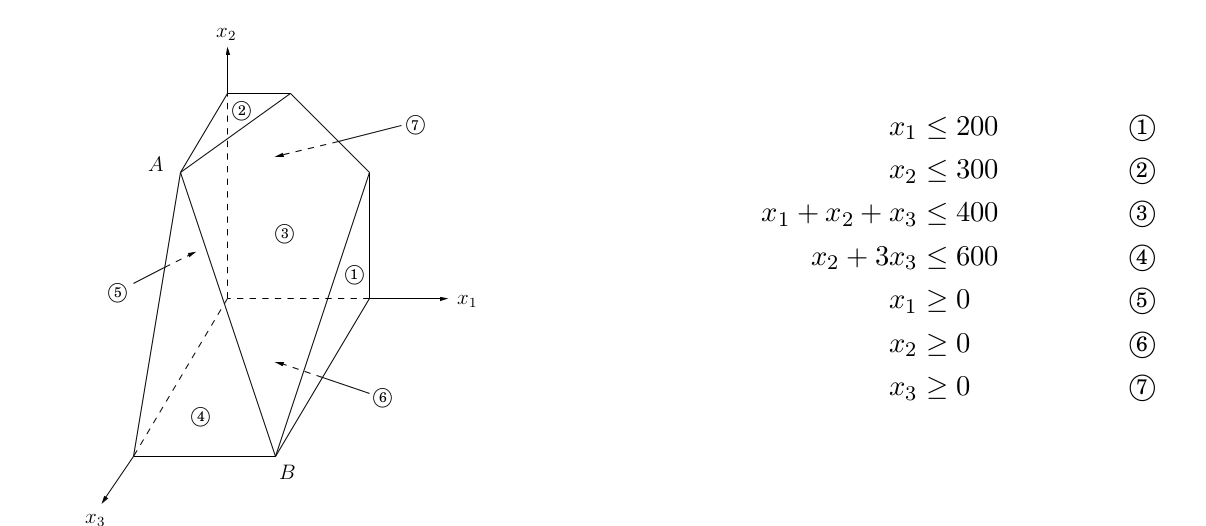
\includegraphics[width=14cm]{PolyhedronDimension/DegeneratedVertex.png}%
        \end{center}\pn
        
        In the figure, you can see that the vertex labeled with $A$ is fully determined by 
        the planes 2, 3, 4, but it also lays in 5, so you could say that any of the plains sets
        $(2, 3, 4), (2, 3, 5), (2, 4, 5)$ and $(3, 4, 5)$ can determine $A$.\pn
        
        Exactly the same happens to $B$.\pn
        
        The way we are going to get rid of these situations is cutting of edges. As you will see in the
        next figure, we have removed the vertices $A$ and $B$ and we have added a new pair of planes, whose
        equations are not really important now.\pn
        
        \begin{center}
            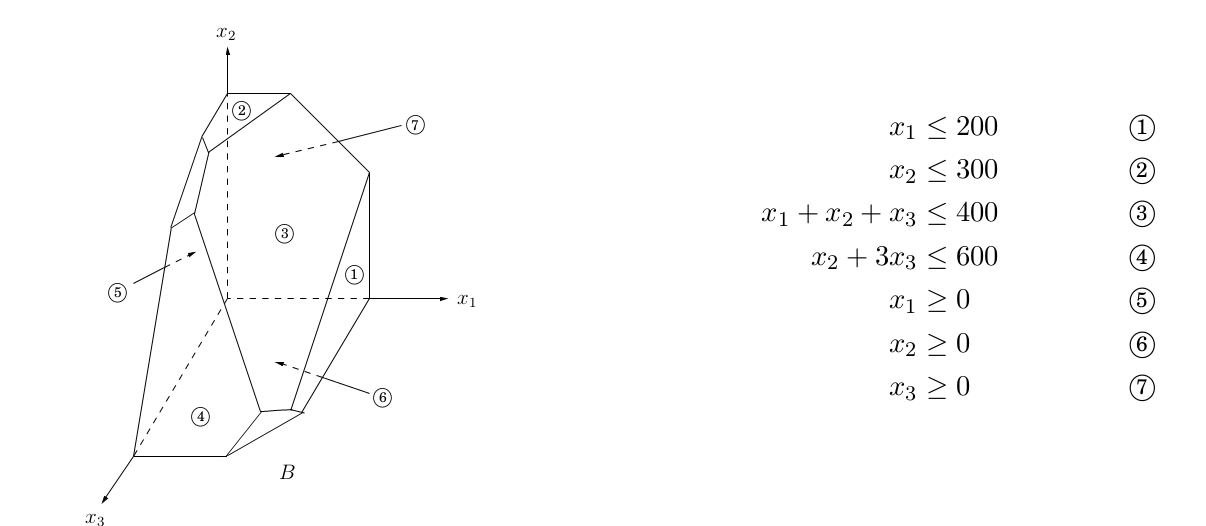
\includegraphics[width=14cm]{PolyhedronDimension/DegeneratedVertex2.png}%
        \end{center}\pn
        
        The important thing now, is that we can remove any degenerated vertex, changing the polyhedron, but not
        its dimension.\pn
        
        So now, we can assume that our polyhedron doesn't have degenerated vertex from the start.\pn
        
        Applying simplex with an auxiliar linear programming problem (adding a new and different variable to each equation),
        we can find a vertex of the polyhedron (unless it is empty). So, lets say that we have already found such vertex and
        lets call it $v$.\pn
        
        We can change our coordinates system in a way that $v$ is the origin of the new system. That is exactly what simplex does
        when is trying to determine if it has reached an optimal value. (That is why we multiply by $B^{-1}$)\pn
        
        Lets say then, that $v = (u_1, u_2, u_3, \dots, u_n) = (0, 0, 0, \dots, 0)$. 
        
        And our linear system will consist now of equations like $u_i \geq 0$, and equations like $(u_1, u_2, \dots, u_n) \cdot (B_1, B_2, \dots, B_n) \leq b$
        For some $B_i$'s and $b$, and as many of these as in the original system.\pn
        
        So, unless we have a condition like $u_i \leq 0$, we can increass $u_i$ as much as some other conditions restricts us, and then, we
        would find a new vertex. This new vertex (lets call it $w_i$) is a neighbor of $v$ and we can collect all the neighbors of $v$ 
        using the same method, only starting with a different $u_i$ each time (a $u_i$ that can be increased).\pn
        
        Lets notice that all these vertex ($v$ and its neighbors) can deffine a convex hull (with interior) that hass exactly the same
        dimension as our original polyhedron.\pn
        
        So, there is the trick, we can get that dimension by simply putting all the neigbors $w_i$ as columns in a matrix $M$ and
        applying gaussian reduction to $M$ to see how many columns (rows) are not zero, and then that number of columns (rows) is our dimension.\pn
        
        But, What would mean that we get zero columns (rows)? That would mean that the neigbors of $v$ are linearly dependent.
        That is that $v$ is a degenerated vertex, but we starting assuming that we do not have degenerated vertices, so we can end
        our algorithm simply by saying that the dimension of our polyhedron is exactly the number of neigbors of $v$. And that is what we are going to do.\pn
        
        So, our algorithm says the next (pseudo code):
        
\begin{lstlisting}
GetPolyhedronDimension(A, b)
    #A is a matrix (n x m), and b is a vector (n x 1).
    #And they define the polyhedron by the linear system
    #A * x <= b
    
    I = Identity(n, n);
    #For the next c, m zeros, followed by n ones.
    auxiliar_c = [0 0 ... 0, 1 1 ... 1];
    Aiuxiliar_problem = [A, I];
    
    v = MinimizeWithSimplex(Auxiliar_problem, b, auxiliar_c);
    
    W = GetNeighborsOfV(A, b, v);
    
    return size(W);
\end{lstlisting}
    \end{proof}